%_____________________________________________________________________________________________
% Chapter 6: Results and Discussion
%_____________________________________________________________________________________________

\chapter{Results and Discussion}
\label{ch:results}

All results in this chapter use logistic regression as the monitored model and a label delay of $L=5$ batches with all labels, unless stated otherwise. Intervals are 95\% bootstrap intervals over episodes. Every number comes from a saved verdict or analysis file in \texttt{artifacts/}; the post hoc analyses are marked as such and do not change any verdict.

\section{v6: The Original Design Fails}
\subsection{Benchmark gate}
The v6 protocol required that at least 25\% of shift episodes on development data be harmful, so that the benchmark would contain enough harm to measure. The gate failed at every allowed shift strength (\figref{fig:day2}): only 17--19\% of shifts were harmful, and raising the strength from 1.5 to 4.0 did not change this. Shifts of the more important features were no more often harmful than shifts of the less important ones (0.18 versus 0.17). Because no allowed strength passed and forcing harm (for example, shifting towards misclassified rows) would have made the benchmark partly circular, we proceeded at $\lambda_{max}=1.5$ by a decision recorded before any held-out data were generated. This is reported as a deviation.

\begin{figure}[H]
\centering
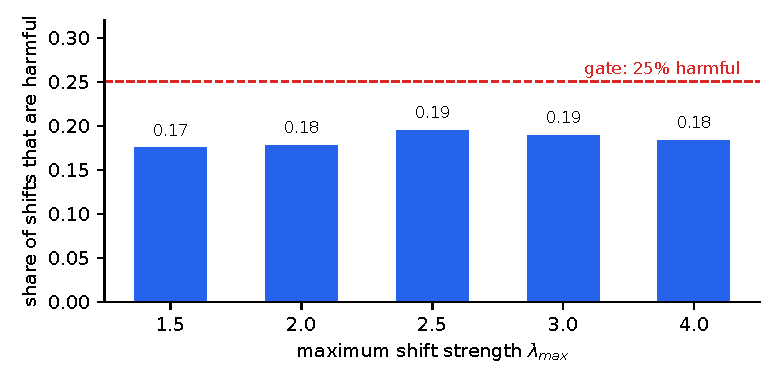
\includegraphics[width=0.75\textwidth]{ch_day2_lambda.pdf}
\caption{Share of development shift episodes that harmed the model, by maximum shift strength. The pre-registered gate required at least 25\%.}
\label{fig:day2}
\end{figure}

\subsection{Pre-registered verdict}
\tabref{tab:v6} shows the verdict on the 5 held-out datasets (53 harmful and 169 harmless shifts). All five hypotheses failed. The learned calibrator warned before the drop on only 22\% of harmful gradual shifts and did not beat waiting for delayed labels. The original DEWS score's higher warning rates on some datasets (\figref{fig:v6ds}) came from alerting almost constantly: on held-out data it raised 36.9 false alerts per 100 clean batches against a budget of 5, while the calibrator raised only 1.2.

\begin{table}[H]
\caption{v6 pre-registered hypotheses on the held-out datasets. Overall verdict: FAILURE.}
\label{tab:v6}
\centering
\small
\begin{tabularx}{\textwidth}{@{}p{5.6cm}Xp{1.25cm}@{}}
\toprule
Hypothesis (target) & Result & Verdict \\
\midrule
H1: T1 on harmful gradual shifts ($\geq$0.60, lead $\geq$2, FA $\leq$5) & 0.22 [0.08, 0.36], lead 12.5, FA 1.2 & Fail \\
H2: T2 gain over waiting for labels ($\geq$0.10, CI $>$0) & 0.83 vs 0.85, $-$0.02 [$-$0.11, 0.08] & Fail \\
H3: harm AUROC ($\geq$0.80); harmless alarms ($\leq$0.10) & 0.59 [0.51, 0.68]; 0.37 & Fail \\
H4: beats the DEWS score ($\geq$4 of 5 datasets) & 2 of 5 & Fail \\
H5: natural streams, T2 gain over labels ($\geq$0) & $-$0.01 [$-$0.08, 0.06] & Fail \\
\bottomrule
\end{tabularx}
\end{table}

\begin{figure}[H]
\centering
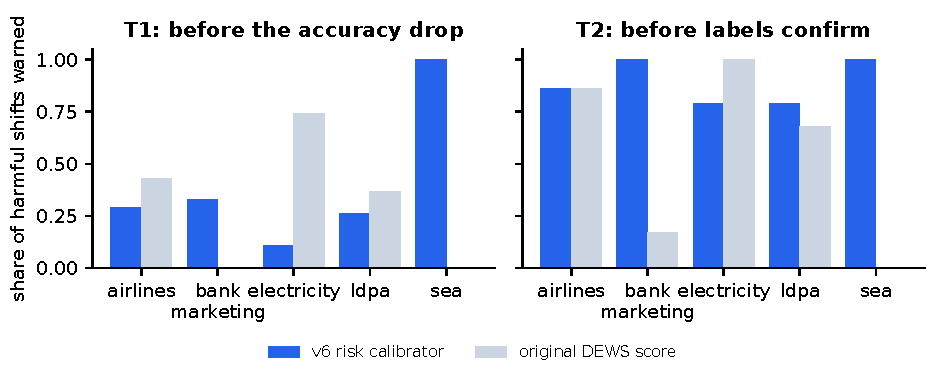
\includegraphics[width=\textwidth]{ch_v6_per_dataset.pdf}
\caption{v6 per held-out dataset: share of harmful shifts warned before the drop (T1) and before labels confirm (T2).}
\label{fig:v6ds}
\end{figure}

\subsection{Secondary settings}
With only 20\% of rows ever labeled (\tabref{tab:scarce}), the gradient-boosting system warned before confirmation more often than the delayed-label trend, but its false alerts exceeded the budget at most delays, and the logistic system stayed below the label trend. We therefore make no claim from these settings.

\begin{table}[H]
\caption{v6 secondary settings with 20\% of labels (held-out): T2 on harmful shifts and false alerts per 100 clean batches.}
\label{tab:scarce}
\centering
\small
\begin{tabular}{@{}lcccc@{}}
\toprule
Model, delay & System T2 & Labels T2 & System FA & Labels FA \\
\midrule
Logistic, $L=0$ & 0.43 & 0.58 & 1.7 & 4.5 \\
Logistic, $L=2$ & 0.38 & 0.57 & 1.0 & 4.0 \\
Logistic, $L=5$ & 0.49 & 0.70 & 1.0 & 5.0 \\
Logistic, $L=10$ & 0.55 & 0.81 & 1.1 & 5.7 \\
Gradient boosting, $L=0$ & 0.64 & 0.48 & 3.9 & 4.0 \\
Gradient boosting, $L=2$ & 0.73 & 0.57 & 5.7 & 5.1 \\
Gradient boosting, $L=5$ & 0.73 & 0.61 & 5.3 & 4.9 \\
Gradient boosting, $L=10$ & 0.82 & 0.80 & 7.7 & 5.9 \\
\bottomrule
\end{tabular}
\end{table}

\section{Why v6 Failed: Thresholds in Raw Units Do Not Transfer}
\figref{fig:transfer} compares, for each method, the false-alert rate on development data (where its threshold was chosen) with the rate on data never used for threshold selection. Scores in dataset-specific units broke the budget by a factor of 3.5--9 (fused DEWS score 4.4 $\rightarrow$ 36.9; mean KS 4.4 $\rightarrow$ 44.6), while the learned calibrator under-alerted (4.6 $\rightarrow$ 1.2). Scores expressed relative to the stream's own normal (drift watch, 2.3 $\rightarrow$ 4.4) or in accuracy points (harm tier, 3.4 $\rightarrow$ 2.8) stayed within the budget on their confirmation data. An ablation of the v6 calibrator confirmed the same mechanism inside the model: removing the raw disagreement levels, which differ widely across datasets, raised its T1 from 0.22 to 0.42. It did not hold everywhere, though. The drift watch broke the budget on natural streams, and the harm tier on the v10 datasets (Section~\ref{sec:followups}).

\begin{figure}[H]
\centering
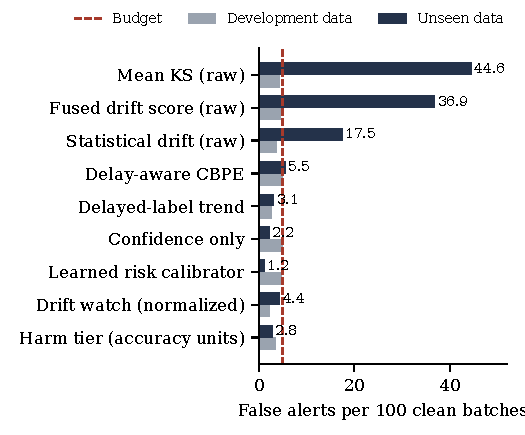
\includegraphics[width=0.8\textwidth]{transfer.pdf}
\caption{False alerts per 100 clean batches with thresholds chosen on development data, on development and on unseen data (v6 held-out data for the v6 methods; v7 and v8 confirmation data for the drift watch and the harm tier). Dashed line: budget of 5.}
\label{fig:transfer}
\end{figure}

\section{v7: The Drift-Watch Tier}
On six fresh datasets (39 harmful gradual shifts) the drift watch warned before the accuracy drop on \textbf{0.87} [0.77, 0.97] of harmful gradual shifts, a median of \textbf{6 batches} ahead, with \textbf{4.4} false alerts per 100 clean batches, and beat the fused DEWS score on 5 of 6 datasets (\tabref{tab:v7}, \figref{fig:v7m}, \figref{fig:v7ds}). Its pre-confirmation warning rate (1.00 against 0.96 for waiting for labels) did not reach the pre-registered gain of 0.10. It also alerted on 96\% of harmless shifts, so it detects drift but cannot tell whether the drift is harmful.

v7 also pre-registered a second tier, a logistic calibrator over the normalised signals. It failed its separation hypothesis (AUROC 0.59, alerts on 53\% of harmless shifts), which motivated the reference-based harm tier of v8.

\begin{table}[H]
\caption{v7 pre-registered hypotheses on six fresh datasets. Overall verdict: PARTIAL SUCCESS.}
\label{tab:v7}
\centering
\small
\begin{tabularx}{\textwidth}{@{}p{5.6cm}Xp{1.25cm}@{}}
\toprule
Hypothesis (target) & Result & Verdict \\
\midrule
C1: WATCH T1 ($\geq$0.60, lead $\geq$2, FA $\leq$5) & 0.87 [0.77, 0.97], lead 6, FA 4.4 & Pass \\
C2: WATCH T2 gain over labels ($\geq$0.10, CI $>$0) & 1.00 vs 0.96, 0.04 [0.00, 0.10] & Fail \\
C3: WARNING separates harm (AUROC $\geq$0.80, harmless $\leq$0.10) & AUROC 0.59; harmless 0.53 & Fail \\
C4: WATCH beats the DEWS score ($\geq$70\% of datasets) & 5 of 6 & Pass \\
C5: natural streams, T2 gain over labels ($\geq$0) & 0.44 vs 0.87, $-$0.43 [$-$0.53, $-$0.32] & Fail \\
\bottomrule
\end{tabularx}
\end{table}

\begin{figure}[H]
\centering
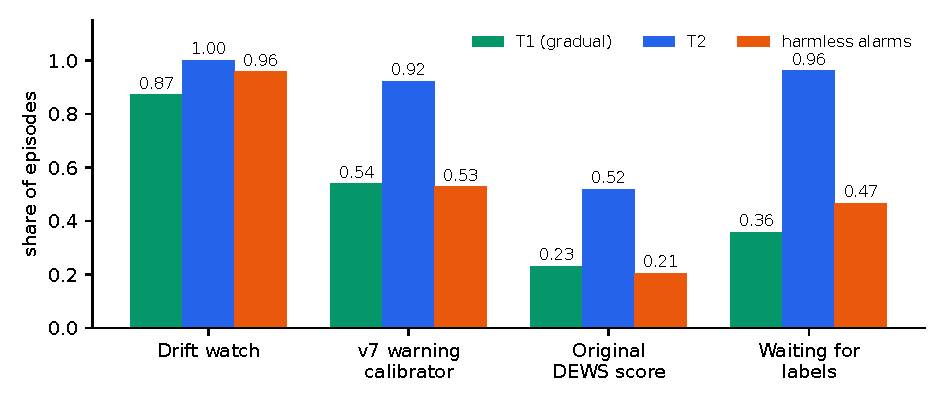
\includegraphics[width=\textwidth]{ch_v7_methods.pdf}
\caption{v7 confirmation data: early warning (T1), pre-confirmation warning (T2) and harmless-shift alarms of each method.}
\label{fig:v7m}
\end{figure}

\begin{figure}[H]
\centering
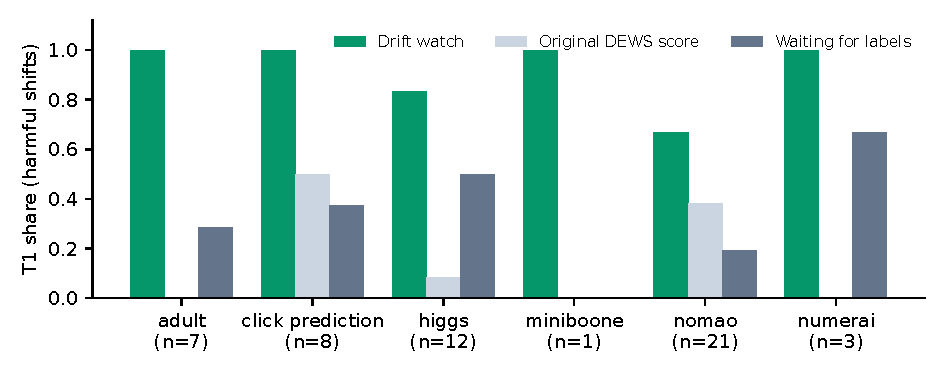
\includegraphics[width=\textwidth]{ch_v7_per_dataset.pdf}
\caption{v7 per confirmation dataset: T1 share of harmful shifts ($n$ = number of harmful shifts).}
\label{fig:v7ds}
\end{figure}

\subsection{Natural streams}
On the 328 natural-stream windows the drift watch failed (T2 0.44 against 0.87 for the label trend) and exceeded the budget (8.0 false alerts per 100 clean batches against 6.3 for the label trend). The data show why. The median degradation began at batch 8, right at the end of the burn-in, and 100 of the 132 events began within 5 batches after it. Accuracy also varied within the burn-in itself (coefficient of variation about 0.12), so the burn-in was not a normal period. Stream normalisation needs a genuinely stable period after deployment.

\section{v8: The Harm Tier}
On five further fresh datasets (64 harmful and 160 harmless shifts) the harm tier cut alarms on harmless shifts from \textbf{0.97} (drift watch) to \textbf{0.34}, while still warning before labels could confirm on 0.83 of harmful shifts and before the drop on 0.76 of harmful gradual shifts, at 2.8 false alerts per 100 clean batches (\tabref{tab:v8}). It separated harmful from harmless shifts with an AUROC of \textbf{0.78} [0.70, 0.86], against 0.59 for the drift watch (gain 0.20 [0.09, 0.30]). It passed two of four hypotheses and missed the AUROC target of 0.80 and the harmless-alarm target of 0.10.

\begin{table}[H]
\caption{v8 pre-registered hypotheses on five fresh datasets. Overall verdict: PARTIAL SUCCESS.}
\label{tab:v8}
\centering
\small
\begin{tabularx}{\textwidth}{@{}p{5.6cm}Xp{1.25cm}@{}}
\toprule
Hypothesis (target) & Result & Verdict \\
\midrule
D1: HARM separates harm (AUROC $\geq$0.80) & 0.78 [0.70, 0.86] & Fail \\
D2: HARM rarely alerts on harmless shifts ($\leq$0.10, FA $\leq$5) & 0.34, FA 2.8 & Fail \\
D3: cuts harmless alarms vs WATCH ($\geq$0.30) with T2 $\geq$0.50 & 0.97 $\rightarrow$ 0.34; T2 0.83 & Pass \\
D4: ranks harm better than WATCH (gain $\geq$0.10, CI $>$0) & 0.78 vs 0.59, gain 0.20 [0.09, 0.30] & Pass \\
\bottomrule
\end{tabularx}
\end{table}

Per dataset (\figref{fig:v8ds}) the harm tier separated harm well on three of the four datasets that produced harmful shifts and was near chance on \emph{kick}; \emph{mv} produced no harmful shift at all.

\begin{figure}[H]
\centering
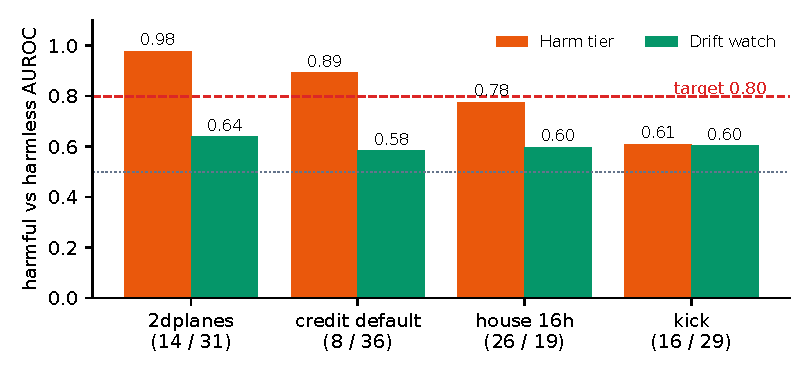
\includegraphics[width=0.85\textwidth]{ch_v8_per_dataset.pdf}
\caption{v8 harmful-versus-harmless AUROC per confirmation dataset (number of harmful / harmless shifts in brackets).}
\label{fig:v8ds}
\end{figure}

\figref{fig:timeline} shows one harmful gradual shift on an unseen dataset. The harm tier first alerts at batch 16, 14 batches before the accuracy event and 20 before delayed labels could confirm it.

\begin{figure}[H]
\centering
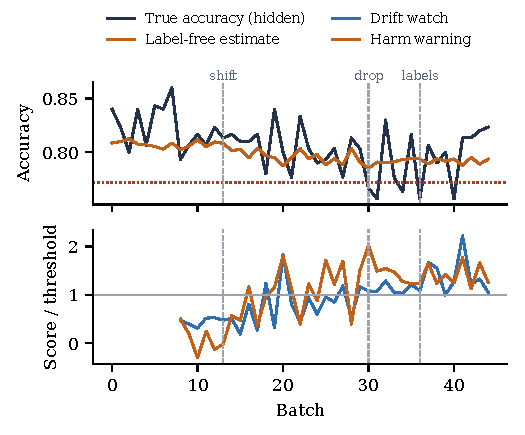
\includegraphics[width=0.8\textwidth]{timeline.pdf}
\caption{A harmful gradual shift on an unseen dataset (credit default, $L=5$). Top: true accuracy (hidden from the monitor) and the label-free estimate; dotted line: 5 points below baseline. Bottom: tier scores divided by their thresholds; above 1 is an alert.}
\label{fig:timeline}
\end{figure}

\section{Same-Data Baselines (Post Hoc)}
To check whether the harm tier is better than simpler label-free estimates, we scored other signals on the v8 confirmation data in exactly the same way (\figref{fig:baselines}). Confidence drop, entropy and delay-aware CBPE reached only 0.56--0.59, and the paired bootstrap interval of the harm tier's advantage over each of them excluded zero. kNN reference accuracy (0.76) and disagreement with models trained on the reference rows (0.73), the other two methods that learn from the labeled reference, were not distinguishable from the harm tier. Confidence drop had reached 0.77 on the v7 data (\tabref{tab:signal_ablation}), so confidence alone is not stable across datasets.

\begin{figure}[H]
\centering
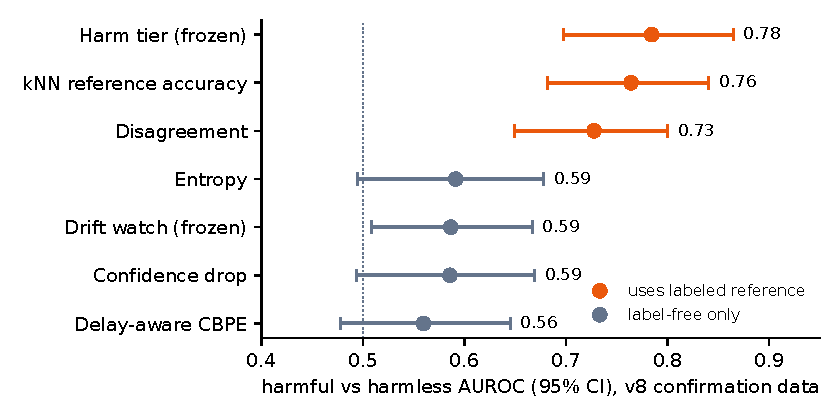
\includegraphics[width=0.8\textwidth]{ch_baselines.pdf}
\caption{Harmful-versus-harmless AUROC of label-free signals on the v8 confirmation data (post hoc), with 95\% bootstrap intervals.}
\label{fig:baselines}
\end{figure}

\section{Why Harmless Shifts Still Alert}
In a post hoc analysis of the v8 confirmation data, streams with no shift at all raised a harm alert in 40\% of episodes and harmless shifts in 34\%, against 88\% for harmful shifts. The harm tier therefore treats harmless shifts like no shift: the remaining alarms are background false alerts that accumulate over about 33 monitored batches. With a per-batch rate of 2.8 per 100, the chance of at least one alert in 33 batches is $1-0.972^{33}\approx 0.6$. Our 10\% target for harmless alarms did not match our own per-batch budget. We noticed this only after the run and left the verdict unchanged.

\figref{fig:operating} shows the full trade-off on the same data. Over most of the range of harmless alarms the harm tier warns on far more harmful shifts than the drift watch. On this data a stricter harm threshold would appear better than the frozen one, but when that idea was frozen and tested on six other datasets (v10, square marker) it warned on only 30\% of harmful shifts. Picking a threshold from this curve after seeing the results would have misled us.

\begin{figure}[H]
\centering
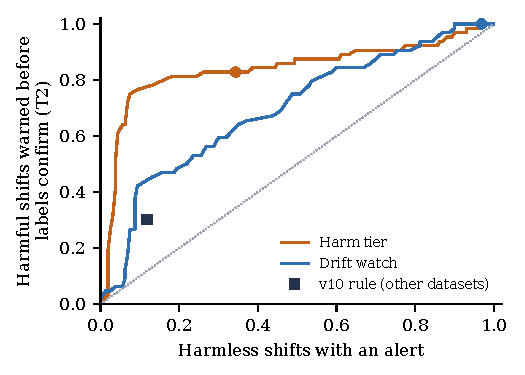
\includegraphics[width=0.75\textwidth]{operating.pdf}
\caption{Post hoc operating curves on the v8 confirmation data; each point is a threshold. Circles: frozen thresholds. Square: the stricter v10 rule, frozen on development data and evaluated on six different datasets.}
\label{fig:operating}
\end{figure}

\section{Pre-Registered Follow-Ups That Failed}
\label{sec:followups}
\textbf{v9: nonlinear harm estimators.} A gradient-boosting domain classifier and an error predictor trained on out-of-fold reference correctness both separated harm worse than the linear estimator on development data (AUROC 0.70 against 0.77). In a post hoc check, ensembles of these estimators, kNN accuracy and confidence (averaging within-dataset ranks) reached at most 0.76. Scored the same way, the linear estimator alone reached 0.75. The 0.80 development gate failed, so no fresh data were used.

\textbf{v10: stricter alerting rules.} Stricter thresholds, exponential smoothing, rolling means, CUSUM, stream-normalised harm scores and gating by the drift watch all reduced harmless alarms at the cost of early warnings. The best rule (a z-scored harm score) passed the development gate, but on six fresh datasets it warned before labels on only 0.30 of harmful shifts against a required 0.50, while reducing harmless alarms to 0.12. Neither v9 nor v10 was adopted.

On the same six v10 datasets the frozen v8 rule warned before labels on 0.74 of harmful shifts but alerted on 58\% of harmless shifts and raised \textbf{12.7} false alerts per 100 clean batches, more than twice the budget. Its calibration therefore did not hold on every new dataset. \figref{fig:tradeoff} places these operating points side by side.

\begin{figure}[H]
\centering
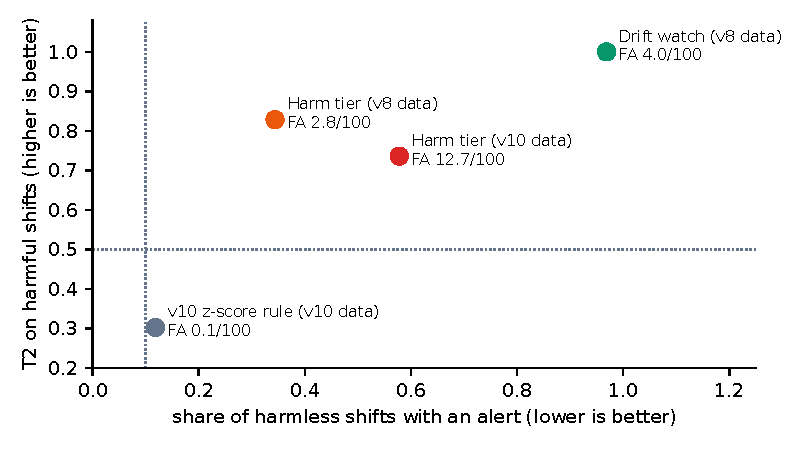
\includegraphics[width=0.78\textwidth]{ch_tradeoff.pdf}
\caption{Harmless-shift alarms against pre-confirmation warnings for the frozen tiers and the v10 rule; FA = false alerts per 100 clean batches.}
\label{fig:tradeoff}
\end{figure}

\section{Ablations}
\subsection{Two families of signals}
Using each normalised signal alone as the drift watch on the v7 confirmation data (\tabref{tab:signal_ablation}, \figref{fig:families}) shows two families with opposite strengths. Input-shift signals warned early on 79--90\% of harmful gradual shifts but could not tell harm from harmlessness (AUROC about 0.5). Model-behaviour signals were harm-aware (AUROC 0.72--0.77) but warned later. Removing any single signal from the drift watch changed little, so no signal is a single point of failure.

\begin{table}[H]
\caption{Each normalised signal used alone (v7 confirmation data, post hoc).}
\label{tab:signal_ablation}
\centering
\small
\begin{tabular}{@{}llccc@{}}
\toprule
Family & Signal & T1 & Harmless alarms & AUROC \\
\midrule
Input shift & fused DEWS score & 0.90 & 0.95 & 0.52 \\
 & mean KS & 0.90 & 0.95 & 0.53 \\
 & relevance-weighted shift & 0.79 & 0.92 & 0.51 \\
 & positive-rate shift & 0.79 & 0.73 & 0.54 \\
Model behaviour & disagreement & 0.49 & 0.42 & 0.72 \\
 & confidence drop & 0.46 & 0.24 & 0.77 \\
 & entropy & 0.41 & 0.25 & 0.75 \\
\midrule
All 7 (drift watch) & & 0.87 & 0.96 & 0.51 \\
\bottomrule
\end{tabular}
\end{table}

\begin{figure}[H]
\centering
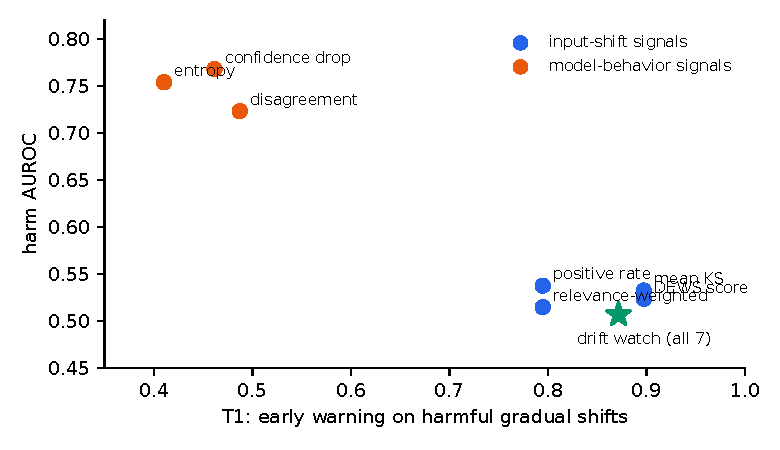
\includegraphics[width=0.72\textwidth]{ch_signal_families.pdf}
\caption{Early warning versus harm separation of each signal used alone (v7 confirmation data).}
\label{fig:families}
\end{figure}

\subsection{Which harm estimator}
All reference-based estimators reached about the same separation on the v8 confirmation data (AUROC 0.76--0.78), far above every drift signal (\tabref{tab:harm_est}). The gain comes from using the labeled reference, not from the particular estimator. The variants trade sensitivity for quietness: nearest-neighbour accuracy is the quietest but warns less.

\begin{table}[H]
\caption{Harm-estimator variants on the v8 confirmation data (thresholds by the separation rule).}
\label{tab:harm_est}
\centering
\small
\begin{tabular}{@{}lccccc@{}}
\toprule
Estimator & T1 & T2 & FA & Harmless alarms & AUROC \\
\midrule
Importance-weighted (frozen) & 0.76 & 0.83 & 2.8 & 0.34 & 0.78 \\
Nearest-neighbour & 0.49 & 0.70 & 0.2 & 0.17 & 0.76 \\
Average of both & 0.71 & 0.83 & 1.0 & 0.29 & 0.78 \\
\bottomrule
\end{tabular}
\end{table}

\subsection{Why most shifts are harmless}
In every data group about 70--80\% of shifts did not harm the model (\figref{fig:harmrates}). Whether harm occurred was barely related to the importance of the shifted feature (the difference appeared only in the v8 group) and not related to the model's baseline accuracy. Harm depends on whether the shift moves data into regions where this particular model is wrong. That explains why feature-importance weighting (v5) failed and why reference-based estimation (v8) was the first approach to separate harmful from harmless shifts.

\begin{figure}[H]
\centering
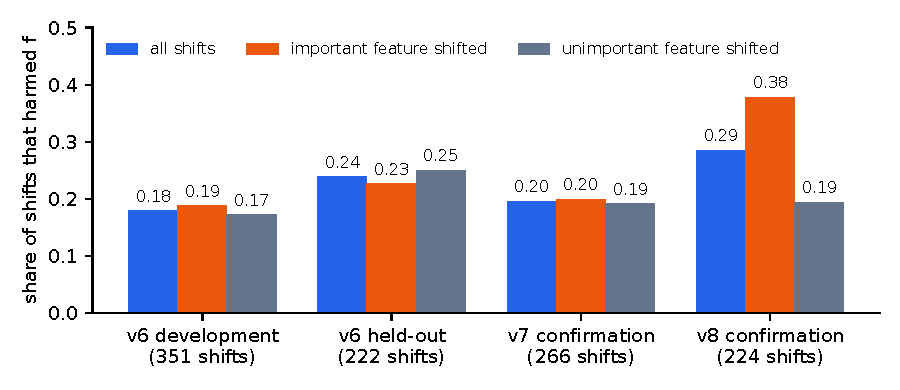
\includegraphics[width=0.9\textwidth]{ch_harm_rates.pdf}
\caption{Share of shift episodes that harmed the model, by data group and by importance of the shifted feature.}
\label{fig:harmrates}
\end{figure}

\section{Discussion}
\subsection{Lessons}
\begin{enumerate}
\item \textbf{Comparable units made thresholds transfer.} The step from v6 to v7 did not need a better model, since the drift watch is simpler than the v6 calibrator; what changed was the scale of the signals. It did not solve everything: the harm rule still broke the budget on the v10 datasets, and the drift watch did on natural streams. Alert thresholds tuned on historical data should be validated on data from other sources before deployment.
\item \textbf{Separate a sensitive drift tier from a specific harm tier.} Input-shift signals are good for early notice; model-behaviour and reference-based signals are needed to judge harm.
\item \textbf{Keep a labeled reference sample.} In our data, only methods that used it separated harm consistently across datasets.
\item \textbf{Make per-episode targets consistent with per-batch budgets.} A 2.8\% per-batch false-alert rate already implies about a 60\% chance of an alarm over 33 batches.
\item \textbf{Several ideas failed on new data.} Online updating (v2), relevance weighting (v5), nonlinear estimators (v9) and stricter rules (v10) all looked useful during development and did not hold up.
\end{enumerate}

\subsection{Threats to validity}
The v7 and v8 designs were motivated by the v6 failure, so they are informed by data we had already seen; we mitigated this by confirming each on datasets downloaded only after its design was frozen, but the sequence of experiments was not planned in advance. The 13 v6 datasets had been explored in v1--v5, so the v6 held-out results are not fully out of sample. Harmful-shift counts per confirmation group (52--64; 39 gradual in v7) give confidence intervals of roughly $\pm$0.1. The event rule (two batches at least 5 points below baseline) and the horizon are conventional choices that we did not vary. Pre-registration was internal (git commits), not on a public registry.

\subsection{Limitations}
Shifts are constructed by re-sampling real rows, which preserves $P(y\mid x)$ and thus favours covariate-shift methods; changes in the label relationship are invisible to every label-free signal until labels arrive. The confirmed model is logistic regression only; the burn-in assumes a stable start, which failed on natural streams; the setting is binary tabular data with 20 features and batches of 300 rows; and the per-dataset numbers of harmful shifts are small, so intervals are wide. The harm tier trains a domain classifier on every batch, and its run-time cost was not measured systematically.
